%! suppress = Unicode
\documentclass[../spec.tex]{subfiles}

\begin{document}

    (A leíró nyelvet hívjuk az egyszerűség kedvéért nahfpa-nak.)
    A formátuma egy egyszerű UTF-8 kódolású szöveges fájl aminek akármilyen kiterjesztése lehet, preferált a \textit{.nah}, vagy a \textit{.math}.
    Egy fájlban, vagy egységben, egy ábrát tudunk leírni, a nyelvnek nem célja a matematikai nyelvi helyességet ellenőrizni.
    A nyelv kifejezéseket tartalmaz, amik balról jobbra olvasva jelennek meg a megjelenítésben, egy kifejezés magában foglalhat gyakran másik kifejezéseket.
    A kifejezések leírása fog következni nyelvtani leírással.
    A fordítás hibával végződik, fordított fájl nem keletkezik ha a fordítónak helytelen nyelvtannal megírt bemenet van adva.

    \subsection{Kifejezésekről álltalánosan}\label{subsec:kifejezésekből-álltalánosan}
    A nyelvben vannak literálisok és parancsok.
    A literálisokat csak be kell írni, és átalakítva megjelennek.
    A parancsok viszont a következő képpen épülnek fel: \lang{\tbs parancs\{paraméter1\}\{parméter2\}...} akárhány paraméterrel.
    A következőkben a \lang{[kif]} helyére akármilyen nyelvtani kifejezés behelyettesíthető.\\
    Vannak parancsok amiknek szükséges valahány darab paraméter, ezeknek az elhagyása fordítási hibát eredményezhet, illetve vannak opcionális paraméterek amelyek minden esetben
    a szükségesek után következnek ezeket a következőkben \lang{[?paraméter]} formában írjuk.
    Az opcionális paraméteter elhagyhatóak a parancs használatakor.\\
    A \{ és \} jelekkel körül tudunk zárni kifejezéseket, hogy azok egy egymás mellé rakott kifejezésként viselkedjenek.
    Pl: \lang{\{a + b + c\}} kifejezés is beírható minden \lang{[kif]} helyére.
    Ez a nyelvtan hasonló lehet egy parancs parméterének megadására, de nem egyenértékűek, tehát például a: \lang{\tbs almaa} az nem az \lang{alma} parancs \lang{a} paraméterrel,
    viszont a \lang{\tbs alma\{a + b\}} parancsban az \lang{\{a + b\}} kifejezés lista a paraméter (Tehát a paraméterek úgy viselkednek, mintha kifejezés listák lennének önmagukban).

    \subsection{Literálok}\label{subsec:szám-literálok}
    Akármilyen ascii karaktersorozat, ami nem tartalmaz whitespace-t illetve operátorokat vagy más nyelvtani elemeket.\\
    Például: \lang{123456}, \lang{3abc} mind úgy jelennek meg ahogy írjuk őket.

    \begin{center}
        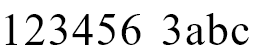
\includegraphics[scale=0.4]{./images/doc1.png}\\
        1. példa
    \end{center}

    \subsection{Egyszerű operátorok}\label{subsec:két-operandusu-egyszerű-operátorok}
    Pontosabban a \textit{+, -, *, /} jelek.
    Ezek akárhogyan elhelyezhetők illetve operandusuk elhagyhatóak. \\
    Például: \lang{[kif] + [kif]}, \lang{** [kif]} (két szorzás operátor egymás mellet aminél az elsőnek nincsen operandusa.) mind helyes kifejezések.

    \begin{center}
        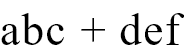
\includegraphics[scale=0.4]{./images/doc2.png}\\
        2. példa
    \end{center}

    \subsection{Szöveg parancs}\label{subsec:szöveges-parancs}
    Akármilyen alfanumerikus karaktersorozatnál ami akár nyelvi elemeket is tartalmaz, akkor garantált a helyes megjelenítés és a whitespace megtartása, ha a \lang{\tbs text\{[szöveg]\}} parancs van használva. \\
    Például: \lang{\tbs text\{almafa, kifli, alma\}} az kiírja, hogy \lang{almafa, kifli, alma}.

    \begin{center}
        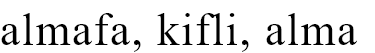
\includegraphics[scale=0.4]{./images/doc3.png}\\
        3. példa
    \end{center}

    \subsection{Emeletes tört parancs}\label{subsec:emelett-parancs}
    A \lang{\tbs frac\{[kif1]\}\{[?kif2]\}} parancs, a \lang{kif1} és \lang{kif2}, kifejezésekből csinál egy emeletes törtet, ahol \lang{kif1} a számláló és \lang{kif2} a nevező.\\
    A parancs két paraméteréből a második elhagyható, ebben az esetben az első paraméter a számlálóba kerül.\\
    Például: \lang{\tbs frac\{123\}\{a + b\}} egy helyes használata a parancsnak.

    \begin{center}
        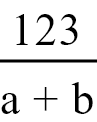
\includegraphics[scale=0.4]{./images/doc4.png}\\
        4. példa
    \end{center}

    \subsection{Gyökjel parancs}\label{subsec:gyökjel-parancs}
    A \lang{\tbs sqrt\{[kif]\}\{[?n]\}} parancs a \lang{kif}-et rakja a gyökjel alá, illetve \lang{n} kifejezést a gyökjel bal indexébe.
    Az opcionális paraméter elhagyásával a bal indexben nem lesz megjelenítve semmi.\\
    Például: \lang{\tbs sqrt\{a + 23\}\{10\}} helyes használata a parancsnak.

    \begin{center}
        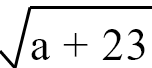
\includegraphics[scale=0.4]{./images/doc5.png}\\
        5. példa
    \end{center}

    \subsection{Felső index operátor}\label{subsec:index-cmd}
    A \lang{[kif1]\tc [kif2]} kifejezésben a speciális \lang{\tc} operátor, a \lang{[kif1]} indexébe helyezi \lang{kif2}-őt.\\
    Fontos megjegyzés: Itt ha kifejezés csoportot akarunk indexbe rakni, vagy annak akarunk az indexébe rakni egy másik kifejezést, használnunk kell a \{ \} szintaktikát.
    Az operátor mindig az azt megelőző első kifejezés-t foglya artumentumnak használni.\\
    Például: \lang{\{alma\}\tc \{a + b\}} egy helyes használata az operátornak.

    \begin{center}
        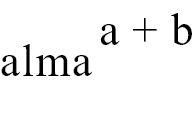
\includegraphics[scale=0.4]{./images/doc6.png}\\
        6. példa
    \end{center}

    \subsection{Alsó index operátor}\label{subsec:subscript-op}
    A \lang{[kif1]\_ [kif2]} kifejezésben a speciális \lang{\_ } operátor, ez \lang{[kif1]} alsó indexébe helyezi \lang{kif2}-őt.\\
    Fontos megjegyzés: A működése teljesen analóg az index operátoréval.\\
    Például: \lang{\{körte\}\_ \{a + b\}} egy helyes használata az operátornak.

    \begin{center}
        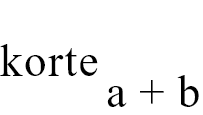
\includegraphics[scale=0.4]{./images/doc7.png}\\
        7. példa
    \end{center}

    \subsection{Index operátor}\label{subsec:index-op}
    A \lang{\tbs index\{[kif1]\}\{[?kif2]\}\{[?kif3]\}} kifejezésben a \lang{[kif1]} felső indexébe helyezi \lang{kif2}-őt és alsó indexébe a \lang{kif3}-at.\\
    Fontos megjegyzés: ez a működés a különálló \lang{\tc, \_} operátorokkal nem reprodukálható.
    Például: \lang{\tbs index\{a\}\{10\}\{20\}} egy helyes használata az operátornak.

    \begin{center}
        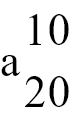
\includegraphics[scale=0.4]{./images/doc8.png}\\
        8. példa
    \end{center}

    \subsection{Szumma parancs}\label{subsec:szumma-parancs}
    A \lang{\tbs sum\{[?felső]\}\{[?alsó]\}} parancs megjelenít egy szumma jelet, ahol a \lang{felső} kifejezés tetején van, az \lang{alsó} kifejezés pedig az alján jelenítődik meg.\\
    Például: \lang{\tbs sum}.

    \begin{center}
        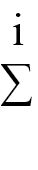
\includegraphics[scale=0.4]{./images/doc9.png}\\
        9. példa
    \end{center}

    \subsection{Produktum parancs}\label{subsec:prod-parancs}
    A \lang{\tbs prod\{[?felső]\}\{[?alsó]\}} parancs megjelenít egy produktum jelet, ahol a \lang{felső} kifejezés tetején van, az \lang{alsó} kifejezés pedig az alján jelenítődik meg.\\
    Például: \lang{\tbs prod}.

    \begin{center}
        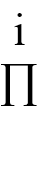
\includegraphics[scale=0.4]{./images/doc10.png}\\
        10. példa
    \end{center}

    \subsection{Szimbólumok}\label{subsec:szimbólumok}
    A következő argumentum nélküli parancsok vannak, amik csak egy szimbólumot jeleníteken meg:
    \begin{itemize}
        \item \tbs int : Integrál
        \item \tbs alpha : Alfa *
        \item \tbs beta : Béta *
        \item \tbs gamma : Gamma *
        \item \tbs epsilon : Epszilon *
        \item \tbs zeta : Dzéta *
        \item \tbs eta : Epszilon *
        \item \tbs theta : Théta *
        \item \tbs iota : Ióta *
        \item \tbs kappa : Kappa *
        \item \tbs lambda : Lambda *
        \item \tbs mu : Mű *
        \item \tbs nu : Nű *
        \item \tbs xi : Kszí *
        \item \tbs omicron : Omikrön *
        \item \tbs pi : Pí *
        \item \tbs rho : Rhó *
        \item \tbs sigma : Szigma *
        \item \tbs tau : Tau *
        \item \tbs upsilon : Üpszilon *
        \item \tbs phi : Fí *
        \item \tbs chi : Khí *
        \item \tbs psi : Pszí *
        \item \tbs omega : Omega *
        \item \tbs le : Kisebb vagy egyenlő
        \item \tbs ge : Nagyobb vagy egyenlő
        \item \tbs neq : Nem egyenlő
        \item \tbs sim : Hullámvonal
        \item \tbs to : Balra mutató kicsi nyíl
        \item \tbs gets : Jobbra mutató kicsi nyíl
        \item \tbs cdot : Szorzó pont
        \item \tbs dots : Három pont (Folytatásnál)
        \item \tbs exists : Létezik
        \item \tbs forall : Mindenre
        \item \tbs approx : Körülbelül egyenlő
        \item \tbs subset : Részhamlaza
        \item \tbs in : Eleme
        \item \tbs cap : Metszet
        \item \tbs inf : Végtelen
    \end{itemize}
    * al jelölt elemek a görög abc betüi, és a megfeleő parancsok nagybetűs formályával lehet a görög abc nagybetűit megkapni pl: \tbs Omega.

    \begin{center}
        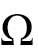
\includegraphics[scale=0.4]{./images/doc11.png}\\
        11. példa
    \end{center}

    \subsection{Limesz parancs}\label{subsec:limesz-parancs}
    A \lang{\tbs lim\{[?alsó]\}} parancs megjelenít egy limesz jelet, ahol az \lang{alsó} kifejezés az limesz aljára kerül.\\
    Például: \lang{\tbs lim\{n \tbs to \tbs inf \} n + 1} matematikailag: n tart végtelenhez, n+1.\\

    \begin{center}
        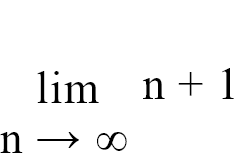
\includegraphics[scale=0.4]{./images/doc12.png}\\
        12. példa
    \end{center}

    \subsection{Kommentek}\label{subsec:kommentek}
    A felhasználó kommenteket helyezhet el a forrásba a \lang{\tbs \#\{[komment]\}} parancs használatával.
    Ez a parancs és tartalma, sehogyan sem fog megjelenni a kimeneti fájlban.

    \subsection{Whitespace}\label{subsec:whitespace}
    A nyelv az összes whitespace karaktert szóközként kezeli.
    Például: \lang{\tbs int[tab]\tbs int} helyes lenne és a kimenete megegyezne a \lang{\tbs int \tbs int} kódrészletével.

\end{document}